\documentclass[11pt,a4paper]{article}

\usepackage[de,break]{ukon-infie}
\usepackage[T1]{fontenc}
\usepackage{lmodern}
\usepackage[utf8]{inputenc}
%\usepackage{pgfgantt} % Timeline 
\usepackage{amsmath}
\usepackage{graphicx}
\usepackage{wasysym}
\usepackage{courier}
\usepackage{textcomp}
\usepackage{hyperref}


\begin{document}
% HEAD |-->
\thispagestyle{empty} %Seitennummerierung 1 ausblenden
\vspace*{5cm} 
\begin{center}
{\huge Software Requirements Specification}\\
{\large Version 1.2}\\
{\large 07. Juni 2013}\\
\end{center}

\begin{center}
{\large ISGCI - Information System on Graph Classes and their Inclusions}\\
{\large Team $Graph$ $Maga$}
\end{center}
% HEAD -->|




%\title{{\LARGE \textbf{Software Requirements Specification}}\\ \textbf{{\large Document}}}
	%\begin{center}
	%\textbf{{\huge Software Requirements Specification}}
	%\end{center}
%\author{\textbf{Graph Maga}}
%\date{\today}
%\maketitle
% \clearpage
 
 
 %
 
 \newpage
 
 % Inhaltsverzeichnis |-->
 \renewcommand{\contentsname}{Inhaltsverzeichnis}
 \tableofcontents % Definiert durch Sections/Subsections
 % Inhaltsverzeichnis -->|

\vfill 
 \section{Änderungsverlauf}

\hspace*{-1cm}
\begin{tabular}{|l|l|p{10.5cm}|}\hline
 \textbf{Version}&\textbf{Datum}&\textbf{Beschreibung der \"Anderung}\\\hline
 1.0&21.05.2013&\textbf{Veröffentlichung}\\\hline
 1.1&23.05.2013& \textbf{Änderungen nach Meeting} \\\hline
   & & Formulierungen \\\hline
 1.2& 07.06.2013 & \textbf{SRS den Aktuellen Mockups anpassen} \\\hline
 & 07.06.2013 &  Einschränkungen ergänzt durch: ISGCI benötigt Internet  \\\hline
  & 07.06.2013 &  Funktionale Anforderungen ergänzt durch:  \\\hline
   &  &  Kontextmenü komplett überarbeitet \\\hline 
    &  &  Selection (Menü-Bar-Parent) ergänzt \\\hline
     &  &  Sidebar hinzugefügt (Mockup) \\\hline
 
 
 
\end{tabular}\\

 \newpage
 
 
 
 
%{\large \textbf{Kommentar (Matze): }

%\textit{Das Dokument ist jetzt nach dem IEEE 830-1998 SRS Standard gerichtet (SE Slides 2-180) und bereits ein wenig modifiziert. Sollte jemand Verbesserungsvorschläge haben, dann kann er sie selbst ändern und/oder mir Bescheid sagen und ich erledige das dann, falls noch nicht geschehen.
%Abgesehen davon sollte man noch überlegen, in welchen Bereich des Dokuments "System Models", "System Evolution", "System Architecture" (Sommerville, Slides 2-178) passen würde.}
%
%\textit{Ich habe jetzt bei jeder Überschrift, sowohl die deutsche als auch englische Überschrift reingeschrieben, die annähernd das selbe beschreiben, vllt kann der ein oder andere mit der anderen Überschrift mehr anfangen, als der andere. Am Ende würde ich sagen entscheiden wir uns für eine Sprache, und da wir das Dokument auf deutsch schreiben wollen, bin ich dafür, dass wir dementsprechend auch die Überschriften deutsch machen. Wenn das nichts ausmachen gern auch englisch, aber dann würde ich das mit Stephan abklären.}
%
%\textit{Die geschweiften Klammern in den einzelnen Bereichen sollen darauf hindeuten, dass dies durch den späteren Inhalt ersetzt werden soll. In den Klammern hab ich versucht, falls möglich zu beschreiben, wie der Inhalt ganz grob aussehen könnte.}
%
%\textit{Ich hoffe, dass aber die Struktur ansonsten allen zusagt.. wenn soweit ist, dann haut diesen Kommentar einfach aus dem Dokument oder kommentiert es im Source-Code aus.. dann kann man nochmal nachschauen, wenn man möchte. }


\section{Einleitung}% / Introduction} % 1. 
%	\{definiere erwartete Leserschaft des Dokuments \& Version History.\\
%    Grund für die Erstellung der neuen Version, bzw. Zusammenfassung der Veränderungen\}



 	\subsection{Zweck} % (des Dokuments)} % / Purpose} %1.1
%	Der Zweck dieses Dokuments ist eine detailreiche Beschreibung des aktualisierten "ISGCI" (Information System on Graph Classes and their Inclusions) Java Projektes. Es wird den Zweck, neue Funktionalität, Interfaces, Einschränkungen und wie es auf externe Einflüsse reagiert. Dieses Dokument ist sowohl für den Kunden als auch für die Entwickler.
	
	Der Zweck dieses Dokuments ist es eine detailreiche Beschreibung des aktualisierten ISGCI-Projektes zu geben. Es wird neue Funktionalitäten, Schnittstellen, Einschränkungen und seine Reaktionen auf externe Einflüsse beschreiben. Dieses Dokument richtet sich sowohl an den Kunden als auch an die Entwickler.
	

  	\subsection{Umfang} % (des Softwareprodukts)} % / Scope} %1.2
   Das gelieferte Produkt ist eine Aktualisierung des bestehenden ISGCI. Das fertige Produkt wird ein Update auf eine neuere Java Version beinhalten. Das bestehende ISGCI wird mit Funktionalität der Graphzeichenbibliothek JGraphX erweitert. Außerdem werden der neuen Version verschiedene neue Funktionalitäten hinzugefügt, die im Punkt 3 genauer beschrieben werden. Zweck des Updates ist es, nicht nur die Funktionalität des Tools in Zukunft zu gewährleisten und neue Funktionen zu implementieren, sondern auch die Instandhaltungskosten zu senken und das Tool für interessierte Entwickler und Nutzer ansprechender zu gestalten.

  	\subsection{Erläuterungen zu Begriffen und Abkürzungen} % (Glossar)}% / Definitions, acronyms and abbreviations} %1.3

	        \begin{itemize}
	        \item[mxGraph] mxGraph ist eine Produktfamilie mehrerer Bibliotheken, die mit verschiedenen Technologien geschrieben sind, welche eine Ausstattung besitzen, mit der interaktive Diagramme und Graphen visualisiert werden können. Zu diesen Bibliotheken gehören unter anderem JGraphX und JGraph (vorige Versionen von JGraphX).
	        \item[ISGCI] Information System on Graph Classes and their Inclusions
	        \item[JGraphT] JGraphT ist eine freie Java Graphenbibliothek, welche mathematische graphentheoretische Objekte und Algorithmen unterstützt. 
	        \item[JGraphX] JGraphX ist eine Java Swing Bibliothek von mxGraph
	        \item[Swing] Swing ist das primäre Java GUI Widget Werkzeug, welche die Bereitstellung von grafische Benutzerschnittstellen ermöglicht.
	        \item[Click\&Drag] Bezeichnet eine Funktion, welche das Greifen und Ziehen von Graphelementen beinhaltet, welche den entsprechenden Graphen manipulieren können.
	        \item[Menu-Bar-Parent] Bezeichnet einen Reiter in der oberen Navigationsbar.
	        \item[Menu-Bar-Child] Bezeichnet ein Item unterhalb des Reiters in der Menu-Bar.
	        \end{itemize}
	        
  	\subsection{Verweise auf sonstige Quellen} % / References} %1.4
  	{
          
          \begin{table}[h]
          	\caption{Verweise}
          	\label{fig:figurename}
          	\begin{center}
          		\begin{tabular}{|l|p{10cm}|c|}
          		\hline
          
          		\hline
          		\textbf{Name} & \textbf{Quelle} & \textbf{Datum} \\
          		\hline
          			 ISGCI & \href{http://www.graphclasses.org/}{Graphclasses.org - ISGCI Homepage} & 13.05.2013\\ \hline
          			 JGraphT & \href{http://jgrapht.org/}{JGraphT Website} & 13.05.2013 \\ \hline
          			 JGraphX & \href{http://www.jgraph.com/}{JGraph Website} & 13.05.2013 \\  \hline
          			  & \href{http://jgraph.github.io/mxgraph/java/docs/index.html}{JGraph Dokumentation} & 13.05.2013 \\  \hline
          			  & \href{https://github.com/jgraph/jgraphx}{JGraphX Library Quellcode} & 13.05.2013\\  \hline
					Swing & \href{http://docs.oracle.com/javase/1.4.2/docs/api/javax/swing/package-summary.html}{Swing Dokumentation} & 13.05.2013 \\  \hline
					Java & \href{http://docs.oracle.com/javase/6/docs/api/}{Java 6 Dokumentation SE} & 13.05.2013 \\  \hline
          		\end{tabular}
          	\end{center}
          \end{table}
          }
    
  	%\subsection{Übersicht/Überblick (Wie ist das Dokument aufgebaut?) / Overview} 1.5
  	%\{Ist dieser Abschnitt notwendig?!.. zur Not einfach kippen\}
  	
\newpage
\section{Allgemeine Beschreibung} % (des Softwareprodukts) / Overall Description} %2.
  	\subsection{Produktperspektive} % (zu anderen Softwareprodukten) / Product Perspective} %2.1
	Unser Produkt wird als Schnittstelle zwischen JGraphX, JGraphT und ISGCI fungieren. Durch die Erweiterung von JGraphX wird dessen Funktionalität verbessert. Mit der Verknüpfung von JGraphX als Zeichenbibliothek werden verschiedene neue Interaktionen ermöglicht und ein Grundbaustein für die Umsetzung des ISGCI als Webapp gelegt. Vor allem, da JGraphX ein OpenSource Projekt ist, verspricht unser Produkt auch in der Zukunft weiterhin neue Funktionen zu erhalten und die Erweiterbarkeit zu vereinfachen.
	%\{Beschreibung, dass unseres Produkt als "Schnittstelle" zwischen JGraphX und ISGCI fungieren wird\\
	%und wie diese miteinander interagieren, bzw. wie darauf aufgebaut wird.\}
  	\subsection{Produktfunktionen} % (eine Zusammenfassung und Übersicht) / Product Functions}  %2.2
  	
	\begin{enumerate}[leftmargin=.9cm]
\item Das System soll einen Graphen zeichnen können, welcher Relationen zwischen Graphklassen zeigt.
\item Das System soll den erzeugten Graphen exportieren können.
%\item Das System soll dazu in der Lage sein eine neue Fensterinstanz zu öffnen.
\item Das System soll die Möglichkeit bieten im gezeichneten Graphen eine Graphklasse zu suchen. 
\item Das System soll dazu in der Lage sein, die Namensgebung der Graphklassen innerhalb des erzeugten Graphen nach vorgegebenen Mustern zu ändern.
\item Das System soll unklare Inklusionen markieren können. (unklare Inklusionen: Beziehungen zwischen zwei Graph-Klassen, bei denen nicht sicher ist, ob die Menge der Graphen der einen Klasse echte Teilmenge der Menge der Graphen der anderen Graphenklasse sind, oder der Menge selbst entsprechen. Keine Information bzgl. $\subset$ / $\subseteq$ in der Datenbank vorhanden.)
\item Das System soll die Graphdatenbank und die Eigenschaften der Graphklassen anzeigen können. 
\item Das System soll die Möglichkeit bieten, nach Relationen zwischen Graphklassen zu suchen.
\item Das System soll die Möglichkeit bieten, zu einem Graph-Problem die entsprechenden Laufzeitklassen zu visualisieren.
\item Das System soll die Möglichkeit bieten, Graph-Probleme im erzeugten Graphen anzuzeigen.
\item Das System soll einen Hyper-Link zu "small graphs" besitzen.
\item Das System soll einen Hyper-Link zur Hilfe Website von ISGCI besitzen.
\item Das System soll eine About Funktion besitzen, welche Versions-, Entwickler- und Software-Informationen enthält.
\item Das System soll die Möglichkeit bieten, einen Knoten im erzeugten Graphen zu markieren.
\item Das System soll die Möglichkeit bieten, einen Knoten im erzeugten Graphen zu verschieben.
\item Das System soll die Möglichkeit bieten, über ein Kontextmenü zu einer Graphklasse im erzeugten Graphen weitere Informationen zu dieser zu erhalten.
\item Das System soll die Möglichkeit bieten, im erzeugten Graphen zu zoomen.
\item Das System soll, wenn ein Graph gezeichnet wird, die für die Zeichnung ausgewählte Graphklasse im Bild zentriert darstellen.
\item Das System soll die Möglichkeit bieten, durch das Gedrückthalten der linken Maustaste und Ziehen den Bildausschnitt zu verschieben.
\item Das System soll Funktionen beinhalten, mithilfe derer man Nachbarknoten beziehungsweise Super- und Subklassen der gewählten Graphklasse ein-/ausblenden kann. Dies soll auch über ein Kontextmenü möglich sein.


\end{enumerate}
     
    \subsection{Benutzermerkmale} % (Informationen zu erwarteten Nutzern, z.B. Bildung, Erfahrung, Sachkenntnis) / User characteristics} %2.3
	Die Zielgruppe des fertigen umgesetzten Systems sind in erster Linie Personen, die sich mit den grundlegenden Eigenschaften von Graphen bereits auskennen und dementsprechend weitere Forschungen zu deren Eigenschaften anstellen wollen. Daher werden viele Grundlagen nicht näher erläutert. Vielmehr sollen sich Personen, die sich mit Zusammenhängen verschiedener Graph-Klassen näher beschäftigen, durch das fertige System einfach Zugang zu Informationen verschaffen können, ohne dass sie weitere Hilfe zur Nutzung des Systems benötigen.
	Letztendlich dient das System also zur Forschung und zum besseren professionellen Verständnis von Graphen.
	%\{Welche Kenntnisse haben die potentiellen Nutzer des Systems, bzw. welche Personengruppen werden das System nutzen.\}    
	\subsection{Einschränkungen} % (für den Entwickler) / Constraints} %2.4
	Die Implementation ist Java-basiert und die Inkompatibilität mit aktuellen Java-Versionen (ab 1.6) erfordert eine Erneuerung des Systems. Dies führt zu verschiedenen Beschränkungen, die beachtet werden müssen.\\
	Die Umsetzung findet für Java-Versionen ab Java 1.6 statt. \\
	Deshalb kann bei niedrigeren Java-Versionen keine Funktionalität gewährleistet werden.\\
	Die graphische Verbesserung des bestehenden Systems wird insbesondere über JGraphX als neue Zeichenbibliothek umgesetzt.\\
	Die Umsetzung findet statt, indem die Funktionalität von JGraph(5) auf JGraphX übertragen wird und anschließend ISGCI an JGraphX angebunden wird.  %Leo: Wie ist das gemeint? JgraphT braucht man also nicht?
	%Dementsprechend ist ausdrücklich gesagt, dass alle Beschränkungen, die für die genannte Bibliothek gelten, insbesondere für die fertige Implementation gelten. \\
	Die Software wird nach Umsetzung auf jedem System ausführbar sein, welches die angegebenen Voraussetzungen erfüllt (Java 1.6 +).\\
	Die Software wird als Open-Source-Project %Englisch nötig?
gehandhabt. Daher wird jede Dokumentation, die zur Erweiterung des Source-Codes stattfindet, in englischer Sprache formuliert, sodass unsere Implementation zur weiteren Nutzung/Forschung beitragen kann. \\
	Des weiteren wird eine Internetverbindung vorrausgesetzt um das ISGCI zu starten. Die Verwendung ist dann ober ohne Internetverbindung möglich.
	%\{zeitliche Einschränkungen (Enddatum der Abgabe), Plattformen, Version, vorgegebene Bibliotheken, Implementationsaufwand, kundenorientiert!!!\}
%	\subsection{Annahmen und Abhängigkeiten (nicht Realisierbares und auf spätere Versionen verschobene Eigenschaften) / Assumptions and dependencies} %2.5 
%	\{Brain-Storming :-)\}
	\subsection{Zuweisung der Anforderungen} %im Gesamten / Apportioning of requirements} %2.6
	Die im nächsten Kapitel beschriebenen funktionalen Anforderungen müssen umgesetzt werden, damit das System bzw. deren Erweiterung die entsprechende Funktionalität hat. Das heißt, dass ISGCI an JGraphX gebunden werden kann und alle bisherigen und hinzukommende Funktionen (außer evtl. Widersprüche) ausgeführt werden können.
\newpage
\section{Spezifische Anforderungen} % (im Gegensatz zu 2.) / Specific requirements} %3.
	\subsection{Funktionale Anforderungen} % (Stark abhängig von der Art des Softwareprodukts)} %3.1
	
	Die bisher vorhandenen funktionalen Anforderungen werden, soweit nicht abweichend angegeben, übernommen.

\vspace*{1cm}
\hspace*{-0.8cm}
\begin{tabular}{|c|p{5cm}|p{10cm}|}
\hline 
 & Name & Beschreibung \\ 
\hline 
1 & Knoten Verschieben & Die Funktion wird dahingehend abgeändert dass ein Knoten vor dem Verschieben markiert werden muss. \\ 
\hline 
2 & Zoom (Mausrad) & Durch das Scrollen mit dem Mausrad wird das Bild gezoomt, Mausrad nach oben entspricht hinein zoomen, Mausrad nach unten entspricht heraus zoomen. \\ 
\hline 
3 & Zoom (Menu-Bar) & Dem Menu-Bar-Parent View werden die Funktionen "Zoom in" und "Zoom out" hinzugefügt, diese können auch per Shortcut ausgeführt werden (alt + +, alt + -). \\ 
\hline 
4 & Fit in window & Der Zoom wird so angepasst, dass der komplette Graph im Canvas sichtbar ist. \\
\hline
5 & Tooltip Werkzeuge& Verweilt die Maus auf einem Menü-Punkt, wird ein Tooltip angezeigt. Der angezeigte Tooltip beinhaltet Informationen zur jeweiligen Funktion. \\ 
\hline
6 & Tooltip Knoten& Verweilt die Maus auf einem Knoten im Graphen, werden alle äquivalenten Graphklassen im Tooltip angezeigt (vgl. Rechtsklick, change name). \\ 
\hline 
7 & Zentrierung & Wird ein neuer Graph gezeichnet ist der zum Zeichnen ausgewählte Knoten im Mittelpunkt des Bildes. \\ 
\hline 
8 & Scrolling / click and drag & Klickt man in den freien Raum und hält die linke Maustaste gedrückt so kann man durch das Bewegen der Maus den angezeigten Bildausschnitt verschieben.\\ 
\hline 
9 & Kontextmenü & Man kann Knoten mit der rechten Maustaste anklicken um ein Kontextmenü zu öffnen. \\
\hline
10 & Kontextmenü Show information & Beinhaltet die bereits vorhandene Funktionalität. \\
\hline
11 & Kontextmenü Show details & Blendet die Sidebar ein. (vgl. Sidebar Punkt 21) \\
\hline
12 & Kontextmenü Change name & Beinhaltet die bereits vorhandene Funktionalität. \\
\hline
13 & Kontextmenü Show neighbours & Kontextmenü-item um vom jeweiligen Knoten alle Nachbarknoten einzublenden. \\
\hline
14 & Kontextmenü Hide neighbours & Kontextmenü-item um vom jeweiligen Knoten alle Nachbarknoten auszublenden. \\
\hline
15 & Kontextmenü Show superclasses &  Kontextmenü-item um vom jeweiligen Knoten alle Superklassen einzublenden. \\
\hline
16 & Kontextmenü Hide superclasses &  Kontextmenü-item um vom jeweiligen Knoten alle Superklassen auszublenden. \\
\hline
17 & Kontextmenü Show subclasses & Kontextmenü-item um vom jeweiligen Knoten alle Subklassen einzublenden. \\
\hline
18 & Kontextmenü Hide subclasses & Kontextmenü-item um vom jeweiligen Knoten alle Subklassen auszublenden. \\
\hline
\end{tabular}
\vspace*{1cm}
\begin{tabular}{|c|p{5cm}|p{10cm}|}
\hline 
19 & Selection (Menu-Bar-Parent) & Es soll einen neuen Reiter in der Menu-Bar geben, der alle Funktionen des Kontextmenüs, außer 12 Change Name, für einen ausgewählten Knoten zur Verfügung stellt (Funktionen 10,11,13-18). Wenn kein Knoten ausgewählt ist, werden alle Child-Items grau dargestellt und besitzten keine Funktionalität.  \\
\hline
20 & Details visible (Menu-Bar-Child) & Im Menu-Bar-Parent View soll ein Punkt Details visible existieren. Dieser signalisiert (mit einem Häkchen) ob, die Sidebar ein- (Häckchen) oder ausgeblendet (kein Häkchen) ist. Außerdem kann über diesen auch die Sidebar ein und ausgeblendet werden.\\ 
\hline
21 & Sidebar & Die Sidebar soll sich durch 3 verschiedene Wege öffnen lassen. Im Kontextmenü über Show details, im Menu-Bar-Parent Selection mit Show details und im Menu-Bar-Parent View über Details visible, falls noch nicht sichtbar. Die Sidebar soll auf der linken Seite sein und wenn nötig eine Scrollbar auf der rechten Seite haben. Die Sidebar wird in ihrer Breite anpassbar sein. Durch einen Button oben in der Sidebar lässt sie sich ausblenden. Außerdem über Details visible in View. Durch das Markieren eines anderen Knoten wird der Inhalt der Sidebar auf die ausgewählte Graphklasse angepasst und deren Informationen in dargestellt. Ist kein Knoten markiert, werden die Informationen der zuletzt ausgewählten Graphklasse angezeigt. Sollte die Sidebar ohne eine Auswahl getroffen zu haben, angezeigt werden, wird die Sidebar leer dargestellt. In der Sidebar wird es möglich sein vertikal in einer Accordion-Navigation zu navigieren. Diese besitzt drei Selektionsmöglichkeiten: Graphclasses, Inclusions, Problems. Dabei führt die Auswahl einer Selektion, zum Einklappen der anderen Selektionsmöglichkeiten. \\
\hline
21 & Sidebar - Selection:Graphclasses  & In der Selection:Graphclasses werden allgemeine Informationen über die ausgewählte Graphklasse angezeigt. \\
\hline
21 & Sidebar - Selection:Inclusions & In der Selection:Inclusions werden Informationen über die Inklusionen der ausgewählten Graphklasse angezeigt. \\
\hline
21 & Sidebar - Selection:Problems & In der Selection:Problems werden die Probleme der ausgewählten Graphklasse angezeigt. \\
\hline
\end{tabular} \newpage

\begin{figure}[htp]
	\begin{center}
		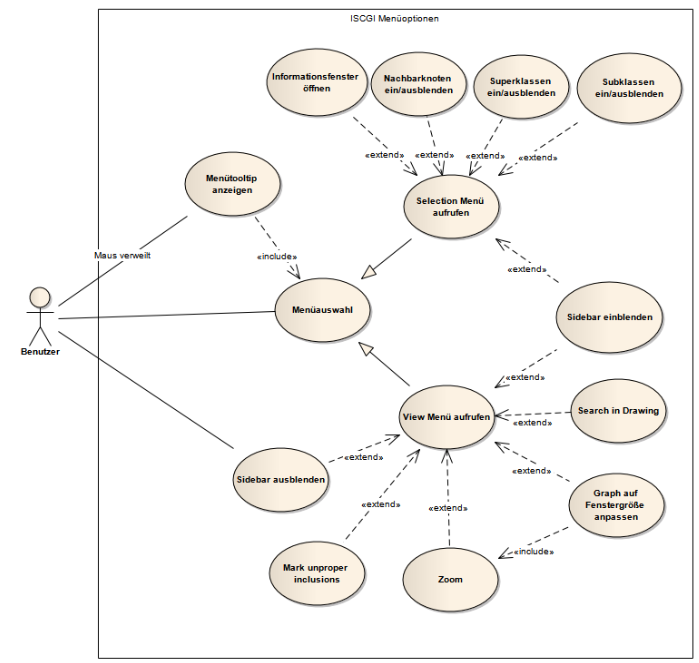
\includegraphics[width=13cm]{Menueoptionen.PNG}\\
	\end{center}
	\caption{Dieses Usecase dient der Veranschaulichung der Interaktionen eines Users mit dem System. Hauptsächlich werden in diesem Usecase alle Interaktionen mit der oberen Menü-Bar dargestellt.}
	\label{fig:figure1}
\end{figure}
\newpage
\begin{figure}[htp]
	\begin{center}
		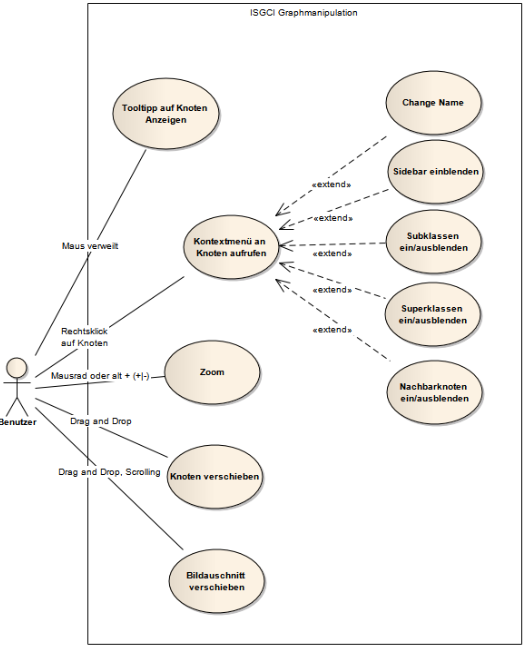
\includegraphics[width=13cm]{Graphmanipulation.PNG}\\
	\end{center}
	\caption{Dieses Usecase zeigt, wie ein Benutzer mit einem Graphen interagieren kann und ihn manipulieren. Dazu gehören Funktionen wie Zoom, Knoten verschieben, Bildausschnitt Verschieben und Tooltips anzeigen.}
	\label{fig:figure1}
\end{figure}

\newpage
\begin{figure}[htp]
	\begin{center}
		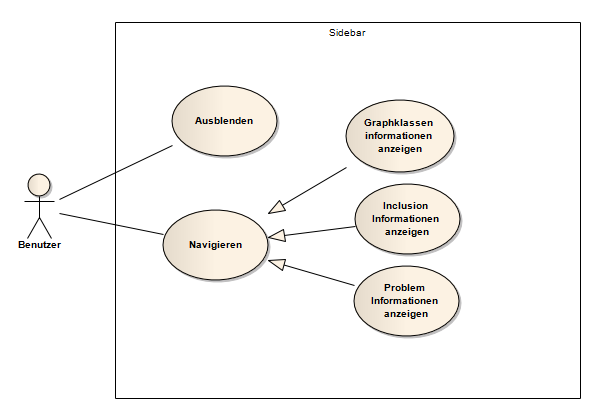
\includegraphics[width=13cm]{Sidebar.PNG}	
	\end{center}
	\caption{Dieses Usecase veranschaulicht die möglichen Interaktionsmöglichkeiten mit der Sidebar, welche neu im ISGCI sein wird.}
	\label{fig:figure1}
\end{figure}
\newpage
\hspace*{10.7cm} Abb. 1

	
	\subsection{Nicht-funktionale Anforderungen} %3.2     
		\begin{itemize}
		\item Technische Grundlage des Softwareprojekts bietet die Programmiersprache Java.
		\item Kompatibilität: Die Software ISGCI wird Java-Runtime-Umgebungen mit Java 1.6 und Nachfolger vollständig unterstützen, solange diese abwärtskompatibel zu Java 1.6 sind. Für ältere Versionen wird die Lauffähigkeit nicht garantiert.
		\item Zur Umsetzung graphischer Anwendungen wird die Grafikbibliothek JGraphX verwendet.
		\item Das Projekt wird als OpenSource veröffentlicht.
		\item Das Benutzerinterface soll interaktiver und userfreundlicher sein als bei der Vorgängerversion (Umsetzung: vgl. Functional Requirements).
		\item Dokumentationen werden auf Englisch verfasst, um sich dem OpenSource Standard und der restlichen Dokumentation anzupassen. Dafür muss der Standard der bisherigen Dokumentation eingehalten werden.
		\item Zeichnungen im ISGCI sollen visuell attraktiver dargestellt werden.
		\item Online Datenbank: Flexible Einspeisung von Datensätzen anstatt statischer Einbindung führt zu einer bessern Wartbarkeit. Auslagerung der Daten auf einen Online-Server statt lokaler Speicherung.
		\end{itemize}
		
	\subsection{Externe Schnittstellen - Anforderungen} %3.3
	\begin{itemize}
	\item[] \textit{Benutzerschnittstellen:}\\
	Der Benutzer benötigt zum vollständigen Nutzen des Systems verschiedene Schnittstellen.\\
	Er benötigt Peripheriegeräte (Maus, Tastatur) und deren Treiberunterstützung entsprechender Hersteller, damit die Funktionalitäten des Systems nutzbar sind.\\
	Der Benutzer benötigt eine grafische Ausgabe (Display/Bildschirm) um das Programm anzeigen lassen zu können. Die Anzeige kann gemäß der benutzerdefinierten Auflösung durch Ziehen des Fensters beliebig angepasst werden.
	\item[] \textit{Hardware Schnittstellen:}\\
	Die fertige Software wird in einer Java-Umgebung dargestellt. Daher wird gefordert, dass die Hardware mit der Java-Umgebung ab der in den nicht-funktionalen Anforderungen genannten Version 1.6 kompatibel sein muss, damit die Software reibungslos funktionieren kann.
	\item[] \textit{Software Schnittstellen:}
	\begin{itemize}
	\item[JGraphX:] Eine Java Swing Visualisierungsbibliothek von mxGraph. 
	\item[ISGCI:] Eine bereits umgesetzte Graphenbibliothek, welche viele Informationen über verschiedene Graphklassen beinhaltet (wie Sub-/Superklassen) und ausführliche Informationen derer Eigenschaften.
	\item[JGraphT:] Eine freie Java Klassenbibliothek, die mathematische graphentheoretische Ziele und Algorithmen unterstützt. Diese läuft allerdings nur auf der Java 2 Plattform, welche mindestens JDK 1.6 voraussetzt.
 	\end{itemize}
	Die Software wird eine Schnittstelle zwischen diesen %beiden 
Bibliotheken bilden, indem die \newline Graphzeichnungsmöglichkeiten von JGraphX genutzt werden. Dementsprechend werden die aktuellen Funktionen von ISGCI, die bis dato mit JGraph umgesetzt sind, auf JGraphX übertragen, indem eine Schnittstelle zwischen JGraphT und JGraphX umgesetzt wird und deren Funktionalität dann von ISGCI auf JGraphX über diese Schnittstelle übertragen wird. 
	
	JGraphT verwendet Maven um den Build Process zur Kompilierung der Java-Klassen und um eine gute Dokumentation zu gewährleisten. Insbesondere führt Maven JUnit-Tests aus, um die Kontrolle über die Implementierung zu behalten. Dazu müssen entsprechende Tests vom Entwickler definiert werden.
	\end{itemize}
	
%	\subsection{Design Constraints (ja das englisch war so vorgegeben und darf gerne geändert werden :-)} %3.4
%	\{Design constraints -- required implementation language, database integrity, limits on usage of resources such as memory, and others.
%	\}
	
	%\subsection{Anforderungen an Performance} %3.5
		
		% KOMMENTAR Keine Änderungen an Performance, Laufzeiten?! - einzige änderung: Graphische Darstellung --> nonfunctional requirements %
		
	%	\{schnelle Laufzeit, wie aktuelles System, damit Änderungen sofort sichtbar sind $\Longrightarrow$ evtl. auch in nicht-funktionalen Anforderungsbereich Punkt 3.2 verschieben!\}
	
	\subsection{Qualitätsanforderungen} %3.6 / Software System Attributes
		\begin{itemize}	
		\item \textbf{Benutzerfreundlichkeit}\\
		Das bestehende System wird vor allem erweitert, um die Benutzerfreundlichkeit zu steigern. Zwar besteht ein Teil der Zielgruppe für die Software aus technisch interessierten und fähigen Personen, dennoch gibt es auch eine breite Nachfrage im Bereich der Computer-Laien, weshalb die Software auch für diese leicht durchschaubar und selbsterklärend sein soll. Intuitiv angeordnete Reiter in der Menüleiste, sowie ein interaktives Kontextmenü sollen dazu beitragen, dass benötigte Funktionen von Benutzern leicht gefunden werden können. Des Weiteren sorgen Funktionen wie Grab\&Pull oder Zoom \textit{(vgl. Funktionale Anforderungen)} für einen interaktiven Umgang mit dem System. Um die Übersichtlichkeit über komplexere Graphen zu gewährleisten, gibt es zwei Varianten des Expanding/Collapsing, mit denen man einen komplizierten Graphen in einen überschaubaren Teilgraphen herunterbrechen kann \textit{(vgl. Funktionale Anforderungen 08)}.
		\item \textbf{Integrität}\\
		Alle Datensätze werden zentral auf einem Server gehalten. Die Software bietet ausschließlich lesende Funktionen an. Somit ist die Datenbank durch negative Manipulationen geschützt.
		\item \textbf{Flexibilität}\\
		Nutzer können ihren Wunschgraphen zeichnen lassen, diesen auf verschiedene Arten manipulieren (z.B.: neu anordnen, reduzieren, Knoten-Hierarchien anzeigen lassen) und den entstandenen Graphen exportieren. Dazu lassen sich zu jedem Graph-Knoten (Graphklasse) Informationen aus der Online-Datenbank einsehen. 
		\item \textbf{Portabilität}\\
		ISGCI ist eine Java Anwendung. Das bedeutet, dass sie plattformunabhängig ausgeführt werden kann, solange eine Java-Laufzeit-Umgebung installiert ist (als Standard vorausgesetzt).
		Die Online-Datenbank ist unabhängig von unserem System. 
		\item \textbf{Wartbarkeit}\\
		Dadurch, dass die Datenbank des Programmes online, zentral gelagert wird, lassen sich Datensätze leicht und ohne Updates im Programm manipulieren oder hinzufügen.
		\end{itemize}
		
%	\subsection{Sonstige Anforderungen} %3.7
%	Other -- database, operations, site adapting, and so on.
%	\subsection{Ergänzende Kommentare} % 3.8
\end{document}
